\documentclass[utf8]{article}
\usepackage{amsmath,amssymb}
\usepackage{graphicx}
\usepackage{fullpage}
\usepackage{setspace}
\usepackage{verbatim}

\usepackage{algorithm}
\usepackage{algorithm}
\usepackage{algorithmicx}
\usepackage{algpseudocode}
\usepackage{amsmath}
\usepackage[top=2cm, bottom=2cm, left=2cm, right=2cm]{geometry}

\onehalfspacing

\title{\bf\huge Lab3 Design Document}
\author{Mei Yixuan 2019011041 Yao92}
\date{\today}

\renewcommand{\algorithmicrequire}{\textbf{Input:}}  
\renewcommand{\algorithmicensure}{\textbf{Output:}} 

\begin{document}
\maketitle

\section{Advanced Cache Replacement Policies}

\subsection{LRU-LIP}
In LRU-LIP, we set counter of the newly inserted block as the number of valid ways in the corresponding set minus one. This ensures that newly added blocks are in the least important position. Also, the counters are continuous (i.e. if we have 3 valids ways, their counters have value 0, 1 and 2). This nice property makes eviction and reversion much easier: we can simply use the same function as in LRU. The hardware control overhead of LRU-LIP is one counter each way, which is identical to LRU. Exact hardware cost is in the following figure.
\begin{figure}[h]
	\centering
	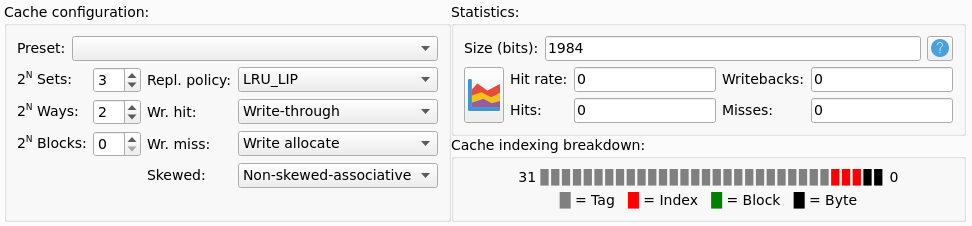
\includegraphics[width=0.7\linewidth]{screenshot001}
	\caption{LRU-LIP hardware cost}
	\label{fig:screenshot001}
\end{figure}


\subsection{DIP}
In DIP, we use the first set (SET0) as MIP sample and the second set (SET1) as LIP sample. In each memory access on non-dueling sets (i.e. sets other than SET0 and SET1), we update cache control fields according to current better replacement policy. We reset all counters every 100000 memory accesses to avoid potential risk of overflow. Thanks to the good property of LRU-LIP, eviction and reversion of DIP is also identical to LRU. Besides the counter in each way, DIP also needs five counters for data recording. Exact hardware cost is in the following figure.
\begin{figure}[h]
	\centering
	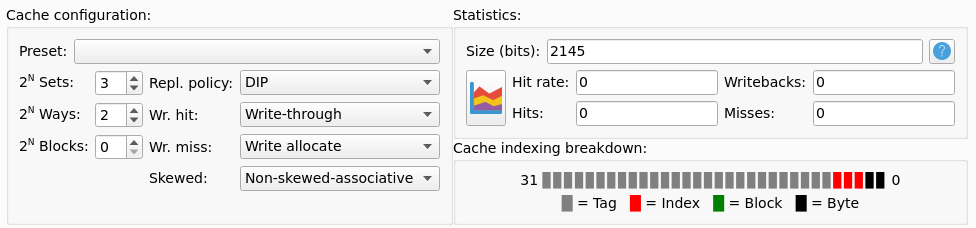
\includegraphics[width=0.7\linewidth]{screenshot002}
	\caption{DIP hardware cost}
	\label{fig:screenshot002}
\end{figure}
\newpage

\subsection{RRIP}
In RRIP, we use counter field of each way to store its RRI. It has field width of 3 bits. Upon hit, we set RRI of corresponding entry as 0. Upon insertion, we set RRI of corresponding entry as long RRI (i.e. 6). When choosing a block for eviction when all ways are occupied, we choose the block with largest RRI and normalize all values to distant RRI (this is identical to adding one repeatedly). Exact hardware cost is in the following figure.
\begin{figure}[h]
	\centering
	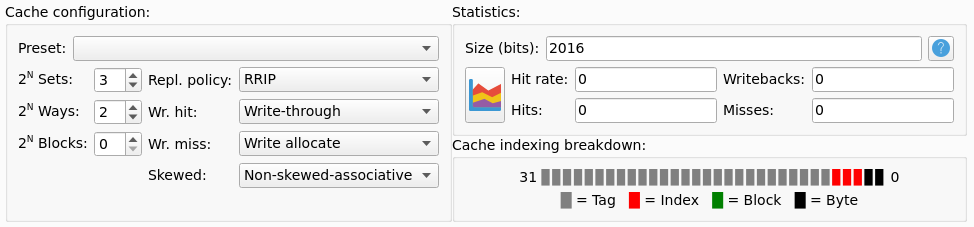
\includegraphics[width=0.7\linewidth]{screenshot003}
	\caption{RRIP hardware cost}
	\label{fig:screenshot003}
\end{figure}

\subsection{Results}
Results of different replacement policies:
\newline

\resizebox{\textwidth}{20mm}{
\begin{tabular}{|c|c|c|c|c|}
		\hline
		Design & Benchmark 1 Miss Rate & Benchmark 2 Miss Rate & Benchmark 1 Total Cycles & Benchmark 2 Total Cycles \\
		\hline
		No Cache & 100 & 100 & 2083191 & 23508468 \\
		\hline
		Random Replacement & 16.47 & 2.44 & 1230758 & 9275269 \\
		\hline
		LRU Replacement & 13.86 & 1.99 & 1204202 & 9209763 \\
		\hline
		LRU-LIP Replacement & 14.77 & 2.76 & 1213470 & 9322490 \\
		\hline
		DIP-Replacement & 14.66 & 2.27 & 1212268 & 9250427 \\
		\hline
		RRIP-Replacement & 13.71 & 2.24 & 1202611 & 9246016 \\
		\hline
\end{tabular}}
\newline

\noindent
Results of different cache capacities and mapping schemes:
\newline

\resizebox{\textwidth}{40mm}{
\begin{tabular}{|c|c|c|c|c|}
	\hline
	Capacity and Mapping & Benchmark 1 Miss Rate & Benchmark 2 Miss Rate & Benchmark 1 Total Cycles & Benchmark 2 Total Cycles \\
	\hline
	16-entry direct-mapped & 29.71 & 26.23 & 1365868 & 12745909 \\
	\hline
	16-entry 4-way associative & 28.74 & 7.52 & 1356019 & 10016283 \\
	\hline
	16-entry 8-way associative & 29.67 & 3.56 & 1365525 & 9439026 \\
	\hline
	16-entry fully-associative & 30.32 & 3.53 & 1372080 & 9433830 \\
	\hline
	32-entry direct-mapped & 19.01 & 19.73 & 1256732 & 11798043 \\
	\hline
	32-entry 4-way associative & 13.86 & 1.99 & 1204202 & 9209763 \\
	\hline
	32-entry 8-way associative & 12.72 & 1.92 & 1192565 & 9199480 \\
	\hline
	32-entry fully-associative & 12.67 & 1.90 & 1191977 & 9196845 \\
	\hline
	64-entry direct-mapped & 13.80 & 6.51 & 1203530 & 9868691 \\
	\hline
	64-entry 4-way associative & 6.49 & 0.54 & 1128914 & 8997426 \\
	\hline
	64-entry 8-way associative & 6.24 & 0.43 & 1126334 & 8981639 \\
	\hline
	64-entry fully-associative & 6.18 & 0.39 & 1125792 & 8975471 \\
	\hline
\end{tabular}
}
\newpage

\section{Skewed-Associative Cache}

\subsection{Implementation}
In skewed-associative cache, we need separate hash functions for each way. Since we want blocks to be independently and uniformly mapped in each way, we choose a group of universal hash functions for mapping. Specifically, we choose $h_{ab}(k) = (a * k + b) \mod m$, in which $k$ is the block address, $m$ is the number of sets. In order for this group of hash functions to be universal, we need to choose $a$ and $b$ uniformly random for each way. Considering actual performance, we choose $a = 1$ for all ways, and $b$ be a random number for each way. Note that the tag function used for non-skewed cache is not suitable for skewed cache, since multiple blocks with the same tag may be mapped into the same way of the same set. Therefore, we use the whole address field as tag instead.

\subsection{Results}

\section{Benchmarks}
\subsection{Replacement Benchmarks}
\subsection{Writehit Benchmarks}
\subsection{Writemiss Benchmarks}

\section{Ripes Bug Report}

\section{Question Answering}

%\begin{center}
%\includegraphics[width=0.1\textwidth]{trump.jpg}
%\end{center}


\end{document}